% vim: set textwidth=78 autoindent:

\subsection{Complemento Georeferenciador}

% when the revision of a section has been finalized, 
% comment out the following line:
%\updatedisclaimer

El complementeo Georeferenciador es una herramienta para la generación de archivos world para rasters.
Permite referenciar rasters a sistemas de coordenadas geográficas o proyectadas creando un archivo world, o transformando el raster a un sistema de coordenadas nuevo. La técnica básica para georeferenciar un raster es localizar puntos en el raster para los cuales puede determinar en forma precisa sus coordenadas. La fuente de las coordenadas puede ser:

\begin{enumerate}
\item El mismo raster, algunas veces las coordenadas son literalmente `escritas' en l raster. 
En este caso puede capturar las coordenadas manualmente.
\item Otros datos georeferenciados, estos pueden ser datos vectoriales o raster que contengan los mismos objetos espaciales que tiene en el raster que desea georeferenciar. En este caso puedes capturar las coordenadas haciendo clic en el conjunto de datos de referencia cargado en el canvas de mapa de Qgis.
\end{enumerate}

El procedimiento usual para georeferenciar una imagen envuelve el seleccionar múltiples puntos en el raster, especificando sus coordenadas, y eligiendo un tipo de transformación relevante. Basado en los datos de parámetros de entrada, el complemento calculará los parámetros del archivo world. Mientras mas coordenadas provea, mejor será el resultado.

El primer paso es iniciar QGIS y cargar el complemento Georeferenciador (vea la sección 
\ref{sec:load_core_plugin}) y haga clic en el ícono \toolbtntwo{georeferencer}{Georeferenciador} que aparece en la barra de menus de QGIS. El diálogo del complemento georeferenciador aparecerá como se muestra en la figura \ref{fig:georefplugin}.
  
Para este ejemplo, estamos usando un hoja topográfica de Dakota del Sur de la SDGS. Puede despues ser visualizada con el conjunto de datos del location spearfish60 de GRASS. Puede descargar la hoja topográfica de aquí: 
\url{http://grass.osgeo.org/sampledata/spearfish\_toposheet.tar.gz}

\begin{figure}[ht]
\begin{center}
  \caption{Diálogo del Complemento Georeferenciador \nixcaption}\label{fig:georefplugin}\smallskip
  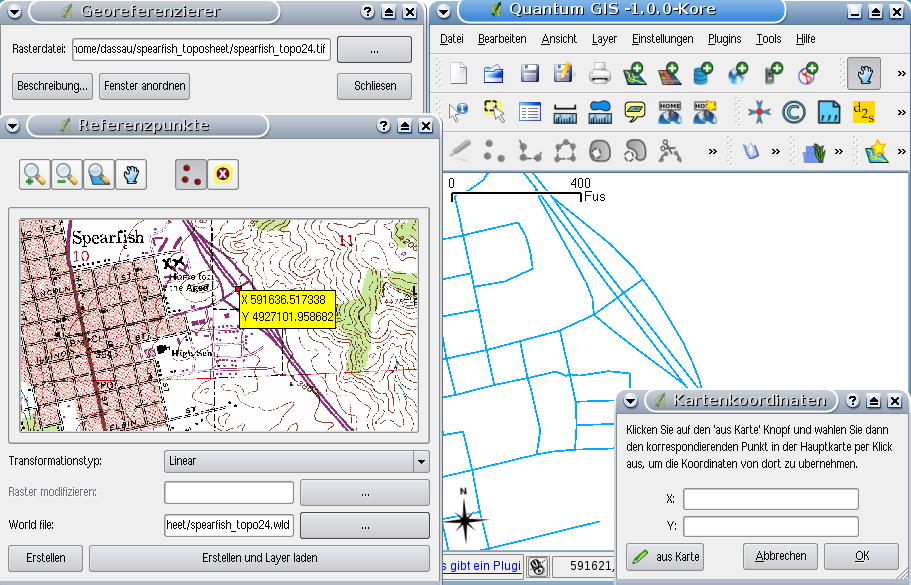
\includegraphics[clip=true, width=12cm]{georefplugin}
\end{center}
\end{figure}

\minisec{Capturando puntos de control de tierra (GCPs)}\label{georeferencer_entering}

\begin{enumerate}
\item Para iniciar georeferenciando un raster no referenciado, debemos cargarlo usando el botón \browsebutton navegar. El raster se mostrará en el área principal de trabajo del dialogo. Una vez que el raster es cargado, podemos empezar a capturar los puntos de referencias.

\item Usando el botón \toolbtntwo{mActionCapturePoint}{Añadir punto}, añada puntos al área de trabajo principal y capture las coordenadas (Vea la figura \ref{fig:choose_points}). Para este procedimiento tiene dos opciones:

\begin{enumerate}
\item Hacer clic en un punto en el mapa raster y capturar las coordenadas X y Y manualmente
\item Hacer clic en un punto en el mapa raster y elegir el botón \toolbtntwo{pencil}{del canvas del mapas} para añadir las coordenadas X y Y con la ayuda de mapa georeferenciado cargado en QGIS.
\end{enumerate}
\item Continue capturando puntos. Debe tener al menos 4 puntos, y mientras mas coordenadas pueda proveer, mejor será el resultado. Hay herramientas adicionales en el diálogo del complementos para hacer zoom y moverse en el área de trabajo para poder localizar el conjuntos de puntos GCP de relevancia.
\end{enumerate}

\begin{figure}[ht]
\begin{center}
  \caption{Añadir puntos a la imagen raster\nixcaption}\label{fig:choose_points}\smallskip
  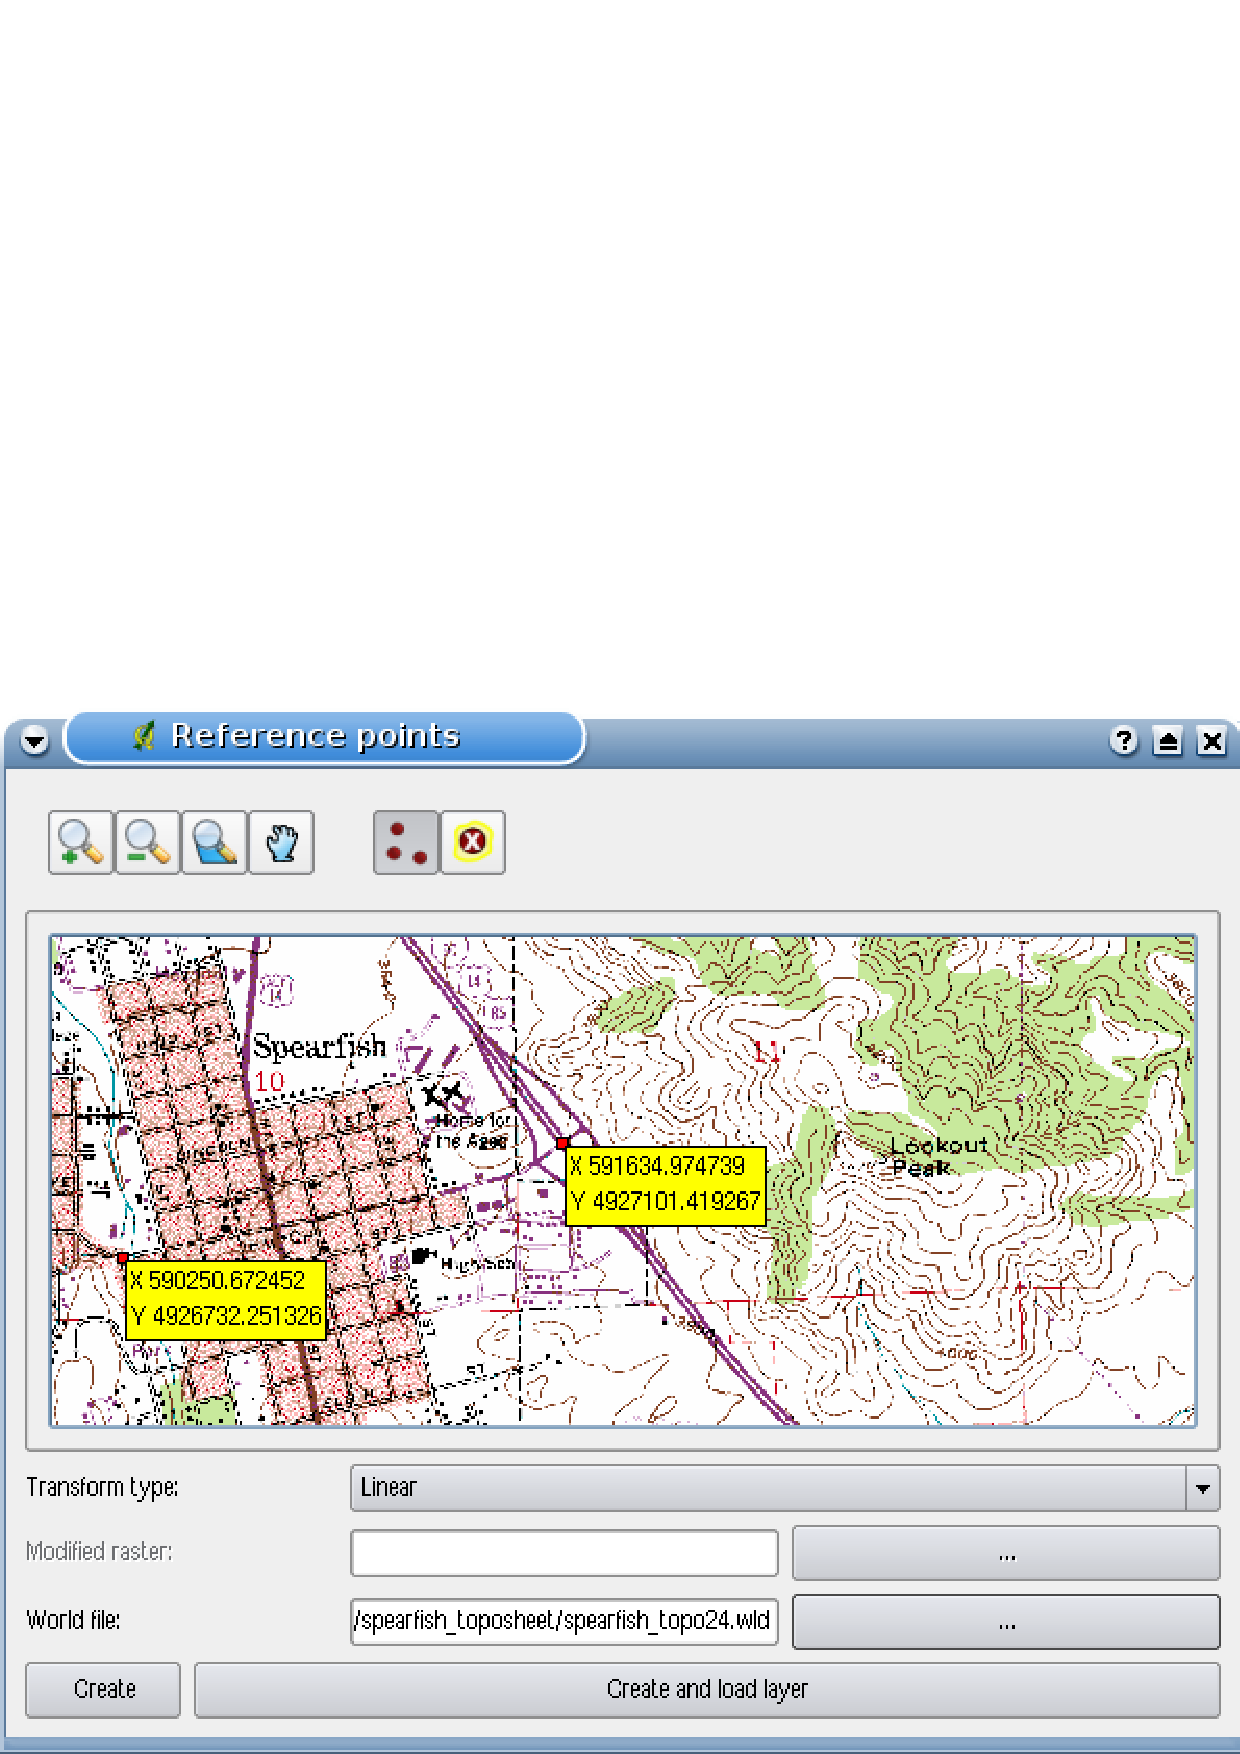
\includegraphics[clip=true,width=9cm]{choose_points}
\end{center}
\end{figure}

Los puntos que han sido añadidos al mapa serán almacenados en un archivo de texto separado ([filename].points) el cual es almacenado junto con la imagen raster. Esto nos permite reabrir el complementos georeferenciados en una fecha posterior y añadir o eliminar puntos para optimizar el resultado. El archivo de puntos contiene valores en la forma de: mapX, mapY, pixelX, pixelY. Puede también \button{Caergar GCPs} y \button{Guardar GCPs} a diferentes directorios si lo desea.

\minisec{Eligiendo la transformación}\label{georeferencer_transformation}

Después de que ha agregado su GCPs a la imagen raster, necesita seleccionar el tipo de transformación para el proceso de georeferenciación. Dependiendo de cuantos puntos de control haya capturado, pudiera utilizar diferentes algoritmos de transformación. La elección del algoritmo de transformación es también dependiente del tipo y calidad de los datos de entrada y la cantidad de distorción geométrica que está desenado introducir al resultado final.

Actualmente, múltiples algoritmos están disponibles:

\begin{enumerate}
\item Linear
\item Helmert
\item Polínomial 1
\item Polínomial 2
\item Polínomial 3
\item Thin plate spline (TPS)
\end{enumerate}

\begin{itemize}
\item El algoritmo lineal es usado para crear un archivo world, y es diferente de los otros algoritmos, ya que no transforma el raster. Este algoritmos probablemente no será necesario si esta tratando con material escaneado.
\item La transformación Helmert realiza transformaciones de escalado simple y rotación. 
\item Los algoritmos polinomiales están entre los algoritmos mas ampliamente usados para georeferenciación, y cada uno difiere por el grado de distorsión introducido para hacer coincidir puntos de control de tierra fuente y destino. El algoritmo polinomial mas ampliamente usado es la transformación de segundo orden, la cual permite un poco de curvatura. La transformación de primer orden polinomial (afín) preserva colinearidad y permite solamente escalamiento, traslado y rotación.
\item El algoritmo Thin plate spline (TPS) es un método de georeferenciación moderno, el cual permite introducir deformaciones locales en los datos. Este algoritmo es útil cuando originales de muy baja calidad están siendo georeferenciados.
\end{itemize}

\minisec{Ejecutando la transformación}\label{georeferencer_running}

\begin{enumerate}
\item Cuando los GCPs han sido recogidos, y la transformación ha sido elegida, presione bien \button{Crear} para crear un nuevo raster o \button{Crear y cargar capas} para agregar automáticamente el nuevo raster a la lista de capas.
\item Un mensaje de alerta aparecerá informándole que un nuevo raster(en formato GeoTIFF) será creado.
\item Después de presionar OK, también le preguntará elegir el método de remuestreo. Hay tres métodos disponibles:

\begin{enumerate}
\item Vecino mas cercano (Nearest neighbour)
\item Lineal
\item Cúbico
\end{enumerate}
\end{enumerate}

\begin{Tip}\caption{\textsc{Eligiendo el método de remuestreo}}
\qgistip{El tipo de remuestreo que elija dependerá de sus datos de entrada y el último objetivo del ejercicio. Si no quiere cambiar estadísticas de la imagen, querrá elegir el remuestreo de Vecino mas Cercano, debido a que el remuestreo Cúbico le proveerá un resultado mas  alisado.}
\end{Tip}


